%\documentclass[12pt]{article}
%\usepackage{amsmath}
%\usepackage{natbib}
%\usepackage[utf8]{inputenc}
%\usepackage{graphicx}
%\usepackage{subcaption}
%\usepackage{float}
%
%%\usepackage{fancyhdr}
%%\fancyhf{}
%%\fancyhead[R]{\thepage}
%
%
%
% \begin{document}
%% \pagestyle{fancy}
%
%\title{C++ Webserver - APK exam project}
%\author{Mikkel Poulsen, Lars Hjerrild, Søren Holm}
%
%\maketitle
%\thispagestyle{empty}
%
%\newpage
%\tableofcontents
%
%
%\newpage\section{Introduction}
%%
%%
%%Eksempler på figure \ref{fig:coffee}
%%
%%Random citation \citep{DUMMY:1} embeddeed in text.
%%
%%\begin{figure}[h!]
%%	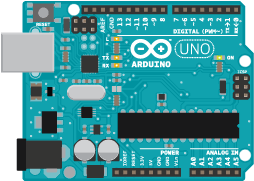
\includegraphics[width=\linewidth]{Figures/Arduino.png}
%%	\caption{Example include.}
%%	\label{fig:examplefig}
%%\end{figure}
%%
%%\begin{figure}[h!]
%%	\centering
%%	\begin{subfigure}[b]{0.4\linewidth}
%%		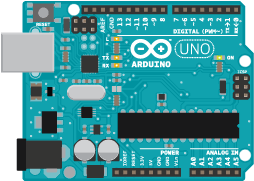
\includegraphics[width=\linewidth]{Figures/Arduino.png}
%%		\caption{Coffee.}
%%	\end{subfigure}
%%	\begin{subfigure}[b]{0.4\linewidth}
%%		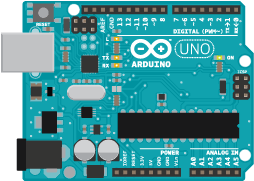
\includegraphics[width=\linewidth]{Figures/Arduino.png}
%%		\caption{More coffee.}
%%	\end{subfigure}
%%	\caption{The same cup of coffee. Two times.}
%%	\label{fig:coffee}
%%\end{figure}\newpage
%%
%% \listoffigures
%% \listoftables
%
% \bibliography{Auto} 
% \bibliographystyle{abbrvnat}
% 
%\end{document}

\documentclass{article}
\usepackage[T1]{fontenc}
\usepackage[utf8]{inputenc}
\usepackage{lmodern}
\usepackage[comma]{natbib}
\usepackage{har2nat}
\usepackage{todonotes}

\bibliographystyle{agsm}
%% or: apsr, dcu, jmr, jphysicsB, kluwer
\usepackage{filecontents}

\begin{filecontents*}{\jobname.bib}
	@incollection{simmons:1980,
		author    = "N. M. Simmons",
		title     = "Behaviour",
		pages     = "124-44",
		year      = 1980,
		booktitle = "The Desert Bighorn",
		editor    = "Gale Monson and Lowell Summer",
		publisher = "University of Arizona Press",
		address   = "Tucson, AZ",
	}
\end{filecontents*}
\begin{document}\pagestyle{empty}
	
	
	
	\title{Anatomi Eksamensprojekt - Fordøjelsessystemet}
	\author{Lars Hjerrild studiednr: 201409555}
	
	\maketitle
	\thispagestyle{empty}
	
	\pagebreak
	\section{Introduction}
	Denne opgave indeholder en anatomisk beskrivelse af de forskellig dele af fordøjelsessystemet. Først vil kirtler og portåresystemet beskrives, og derefter cavitum oris, oesophagus og ventriklen, for til sidst at dykke ned i tarmsystemet.\\
	
	
	\section{Oesophagus}
	Oesophagus som på dansk kaldes spiserøret er et 25 cm langt muskuløst rør, der går fra halsrod til cavitas abdominalis. Undervejs går oesophagus igennem diaphragma ved hiatus oesophagus. I cervix/collum har oesophagus relationer til Gl. thyroidea, trachea og n. Larygeus recurrens \todo{Add more}.\\
	
	Oesophagus løber ligeledes ned igennem thorax hvor den har et andet set af relationer. Posteriort ligger Collumna, og dereter vil man sige at oesophagus havde forskellige relationer ift. hvilken del af mediastinum den lå i.\\
	
	I mediastinum superius ligger Trachea og bifurcaturen anteriort. På højre side ligger pulmones dxt og den dertilhørende pleura, samt v. Azygos. På venstre side af oesophagus ligger a. Carotis cummunis sin, A. Subclavia sin og Argus aorta. Dette er relationerne i medistinum superius.
	
	I medistinum posterius ligger Aorta descendens pars thoracica, Ductus thoracicus og v. Azygos posteriort ift. oesophagus. Der er relationer til begge pulmones og pleura. På venstre side er der ligeledes relation til aorta descendens pars thorcica, og anteriort er der relation til Cor. N. Vagus omspinder i dette område oesophagus som plexus oesophagus.\\
	
	Sidst går oesophagus igennem diaphragma og ender i ventriklens cardia, hvor den anteriort dækkes af Hepa\todo{Look it up}.
	
	 
	 
	\section{Ventriklen}
	Ventriklen eller gastor er det vi på dansk kalder mavesækken. Helt generelt om gastor kan sige at den fungerer som et reservoir for føde. I gastor er der både mekaniske og kemiske mekanismer der hjælper til nedbrydelsen af føde, hvor den kemiske del er saltsyre. Vetriklens placering i abdomen er intraperitonalt, og ellers opad mod venstre i cavitas abdominalis. Ventrikler har to krøs Ventriklen kan opdeles i 4 dele. 
	\begin{enumerate}
		\item Pars Cardia
		\item Fundus ventriculi
		\item Corpus ventriculi
		\item Pars pulorica
	\end{enumerate}
	Der er åbninger til ventriklen ved Cardia, (hvor oesophagus løb ind) og ved Pylorus, som er udgangen til duodenum. Ved sidstnævnte er der en ringmuskel der kan styrer tømningen. Ventriklen har to kanter som er curvatura minor og curvatura major. 
	
	\subsection{Curvatura minor}
	Dette kaldes den lille kant som er ca. 10 cm lang. \todo{add more}
	\subsection{Curvatura major}
	\todo{add more}
	
	Ommentum majus
	
	
	Hvis man ser på ventriklen kan struktur indefra og ud kan man opdele det i. \todo{add opdeling}
	
	\section{Duodenum}
	Duodenum er det vi på dansk kalder for tolvfingertarmen. Denne er ca. 25 cm lang, hvor ca. de første 2 cm er intraperitonaele, og resten er retroperitonealt. Dette betyder også at duodenum ikke har noget krøs. Duodenum kan indeles i fire dele:
	\begin{enumerate}
		\item Pars superior duodeni
		\item Pars descendens duodeni
		\item Pars horisontalis/inferior duodeni
		\item Pars ascendens duodeni
	\end{enumerate}
	
	I Pars descendens findes parpilla duodeni major, som er udmundingen ductus pancreaticus og ductus choledocus. Ligeledes findes her Papilla duodeni major
	
	\pagebreak
	%\citep{simmons:1980}
	\bibliography{\jobname}
\end{document}